\section{熵}
\label{sec:info-entropy}

天气预报说明天有雨，在雨季几乎不值得一提，在旱季却是大新闻。同一句话带来的信息多少，取决于它事先有多意外。本节先给单个结果的意外程度一个数值，再对所有可能结果取平均，得到衡量随机结果不确定性的熵。离散结果可以直接这样做；对有密度的连续结果照搬公式时，会多出一个依赖坐标尺度的量，需要单独说明。

\subsection{自信息}
\label{sec:info-self-information}

设某个结果发生的概率是$p\in(0,1]$。我们想给它指定一个数$c(p)$，表示“得知这个结果发生”所获得的信息量。至少有两个要求是自然的。

第一，越罕见的结果越意外，信息越多，所以$c$是$(0,1]$上的递减函数；必然发生的结果不带来信息，$c(1)=0$。第二，两个独立结果同时发生的概率是$pq$，分别得知它们和一起得知它们，获得的信息应当一样多，所以
\[
  c(pq)=c(p)+c(q),\qquad 0<p,q\leq1.
\]
回到章首的四字母表：结果$c$的概率是$\tfrac18$，它相当于连续三次“二选一”都选中某一边，每次概率$\tfrac12$；按第二个要求，它的信息量应是$\tfrac12$对应信息量的三倍。

\begin{theorem}[自信息的形式]
\label{thm:info-self-information-form}
设$c:(0,1]\to[0,\infty)$递减且对一切$p,q\in(0,1]$满足$c(pq)=c(p)+c(q)$，则存在常数$a\geq0$，使
\begin{equation}
  c(p)=-a\ln p,\qquad 0<p\leq1.
  \label{eq:info-self-information-form}
\end{equation}
\end{theorem}

\begin{proof}
令$b(u)=c(\mathrm{e}^{-u})$，$u\geq0$。指数函数把加法变成乘法，所以$c$的乘法关系变成$b$的加法关系：
\[
  b(u+v)=b(u)+b(v),\qquad u,v\geq0.
\]
$u$增大时$\mathrm{e}^{-u}$减小，$c$递减，所以$b$在$[0,\infty)$上递增。

先看有理点。由可加性，$b(0)=b(0)+b(0)$，故$b(0)=0$；对正整数$n$，$b(nu)=nb(u)$。取$u=1/m$，得$b(1)=m\,b(1/m)$，于是对正整数$n,m$，
\[
  b\Bigl(\frac{n}{m}\Bigr)=n\,b\Bigl(\frac1m\Bigr)=\frac{n}{m}\,b(1).
\]
记$a=b(1)\geq b(0)=0$，则$b(r)=ar$对一切非负有理数$r$成立。

再看一般的$u\geq0$。对任意有理数$r\leq u\leq s$，单调性给出$ar=b(r)\leq b(u)\leq b(s)=as$。让$r,s$从两侧趋于$u$，得$b(u)=au$。代回$u=-\ln p$，即得式~\eqref{eq:info-self-information-form}。
\end{proof}

证明里两个要求各起一个作用：可加性把$c$在有理点上的值全部确定下来，单调性把有理点之间的空隙填满。只有可加性而没有任何正则性时，满足$b(u+v)=b(u)+b(v)$的函数可以极不规则，结论就不再成立。常数$a$不受这两个要求约束，它只决定信息量的单位。

\begin{definition}[自信息]
\label{def:info-self-information}
设离散随机变量$X$的概率质量为$p_X$。对$p_X(x)>0$的取值$x$，称
\begin{equation}
  \iota(x)=-\ln p_X(x)
  \label{eq:info-self-information}
\end{equation}
为结果$x$的\term{自信息}（self-information），单位为\term{奈特}（nat）。若改用$-\log_2 p_X(x)$，单位为\term{比特}（bit）。
\end{definition}

两种单位只差一个正的常数倍：$-\log_2 p=-\ln p/\ln2$，所以
\[
  1\ \mathrm{bit}=\ln2\ \mathrm{nat}\approx0.693\ \mathrm{nat}.
\]
换单位不改变任何两个信息量的大小顺序，也不改变“相等”“为零”这类结论。本章用nat计算，以bit解释“是非题个数”。

比特的说法来自是非题。一个概率为$2^{-k}$的结果，自信息是$k$ bit，恰好相当于连续回答$k$个各占一半的是非题。图~\ref{fig:info-self-information}画出$-\ln p$，右侧刻度换成bit。$p$从$1$减小到$\tfrac12$只带来$1$ bit，而每再减半一次就多$1$ bit；概率趋于零时自信息趋于无穷。

\begin{BookInlineFigure}
  \centering
  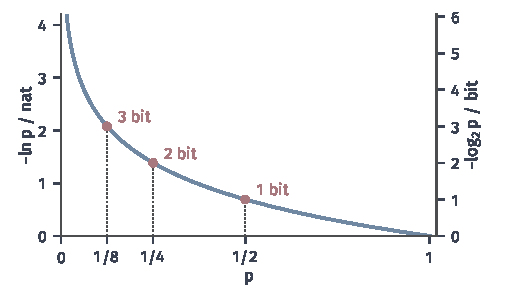
\includegraphics[width=86mm]{figures/07-probability/04-distribution-analysis/matplotlib/info-self-information/figure.pdf}
  \caption{自信息随概率的变化。蓝线为$-\ln p$，左轴以nat计，右轴为同一曲线以bit计的刻度。红点是四字母表中概率$\tfrac12,\tfrac14,\tfrac18$的结果，分别对应$1,2,3$ bit。}
  \label{fig:info-self-information}
\end{BookInlineFigure}

自信息是一次结果的属性。看到罕见结果时获得很多信息，但罕见结果很少出现；要衡量一个随机结果“平均”含有多少信息，还要按概率取平均。

\subsection{离散熵}
\label{sec:info-discrete-entropy}

章首的四字母表可以按图~\ref{fig:info-question-tree}的方式提问。每个结果所需的题数恰好是它以bit计的自信息：$a$一题，$b$两题，$c,d$各三题。平均题数是
\[
  \tfrac12\cdot1+\tfrac14\cdot2+\tfrac18\cdot3+\tfrac18\cdot3=1.75.
\]
这就是自信息的平均。对一般的概率表，题数必须是整数，不一定能与自信息一一相等；第~\ref{chap:lossless-coding}章证明，最好的提问方案平均题数与以bit计的熵相差不到一题。

\begin{BookInlineFigure}
  \centering
  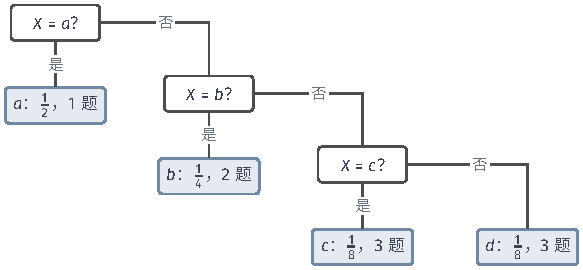
\includegraphics[width=98.7mm]{figures/07-probability/04-distribution-analysis/tikz/info-question-tree/figure.pdf}
  \caption{四字母表$(\tfrac12,\tfrac14,\tfrac18,\tfrac18)$的一种是非题提问方案。蓝框是确定下来的结果，框内为其概率与所需题数；每个结果的题数等于$-\log_2 p$，平均题数为$1.75$。}
  \label{fig:info-question-tree}
\end{BookInlineFigure}

\begin{definition}[离散熵]
\label{def:info-discrete-entropy}
设离散随机变量$X$取值于有限或可数集合$\mathcal{X}$，概率质量为$p_X$。$X$的\term{熵}（entropy）定义为
\begin{equation}
  H(X)=-\sum_{x\in\mathcal{X}}p_X(x)\ln p_X(x)=\mathbb{E}[-\ln p_X(X)],
  \label{eq:info-entropy}
\end{equation}
其中约定$0\ln0=0$。各项非负，和可以为$+\infty$。
\end{definition}

约定$0\ln0=0$有两个理由。概率为零的结果从不出现，不应影响平均；并且$t\ln t\to0$（$t\downarrow0$），约定与极限一致，加入或删去零概率的取值都不改变熵。熵只依赖概率值的集合，与取值叫什么无关：把$a,b,c,d$换成$1,2,3,4$或任意排列，熵不变。这一点与期望、方差不同，后者依赖取值本身。

四字母表的熵为
\[
  H(X)=\tfrac12\ln2+\tfrac14\ln4+2\cdot\tfrac18\ln8=\tfrac74\ln2\approx1.213\ \mathrm{nat},
\]
即$1.75$ bit。若四个字母等可能，熵为$\ln4\approx1.386$ nat，即$2$ bit。

\paragraph{有限字母表上的基本性质}
下面的性质说明熵确实符合“不确定性”的直觉：确定的结果没有不确定性，均匀分布最不确定，把两个分布混合起来不会更确定。

\begin{theorem}[有限字母表上熵的范围]
\label{thm:info-entropy-range}
设$X$取值于$m$个元素的集合$\mathcal{X}$。则
\begin{equation}
  0\leq H(X)\leq\ln m.
  \label{eq:info-entropy-range}
\end{equation}
左边等号当且仅当$X$以概率$1$取某一个值；右边等号当且仅当$X$在$\mathcal{X}$上均匀分布。
\end{theorem}

\begin{proof}
每个$p_X(x)\in[0,1]$，所以$-p_X(x)\ln p_X(x)\geq0$，和非负。各项为零当且仅当$p_X(x)\in\{0,1\}$，而概率之和为$1$，这只能是某一个$x$的概率为$1$。

右边用不等式$\ln t\leq t-1$（$t>0$），它在$t=1$处取等号，其余处严格成立。记$S=\{x:p_X(x)>0\}$。对$x\in S$取$t=1/(m\,p_X(x))$，得到
\[
  H(X)-\ln m=\sum_{x\in S}p_X(x)\ln\frac{1}{m\,p_X(x)}\leq\sum_{x\in S}p_X(x)\Bigl(\frac{1}{m\,p_X(x)}-1\Bigr).
\]
右端化简为
\[
  \sum_{x\in S}\frac1m-\sum_{x\in S}p_X(x)=\frac{\lvert S\rvert}{m}-1\leq0.
\]
等号要求两处同时取等：每个$x\in S$都有$m\,p_X(x)=1$，并且$\lvert S\rvert=m$。这正是均匀分布。
\end{proof}

上界$\ln m$只依赖字母表的大小。它说明熵“用掉”多少个可能结果：熵为$\ln m$的变量与$m$个等可能结果一样不确定。四字母表的$1.213$ nat小于$\ln4$，因为它的质量偏向$a$。

\begin{theorem}[熵的凹性]
\label{thm:info-entropy-concave}
在有限字母表$\mathcal{X}$上，把熵看成概率向量$\bm{p}$的函数$H(\bm{p})=-\sum_x p_x\ln p_x$。对任意两个概率向量$\bm{p},\bm{q}$与$\lambda\in[0,1]$，
\begin{equation}
  H(\lambda\bm{p}+(1-\lambda)\bm{q})\geq\lambda H(\bm{p})+(1-\lambda)H(\bm{q}).
  \label{eq:info-entropy-concave}
\end{equation}
\end{theorem}

\begin{proof}
令$\psi(t)=-t\ln t$（$t>0$），$\psi(0)=0$。在$t>0$处$\psi''(t)=-1/t<0$，$\psi$在$(0,\infty)$上凹，又在$0$处连续，所以在$[0,1]$上凹。对每个坐标，
\[
  \psi(\lambda p_x+(1-\lambda)q_x)\geq\lambda\psi(p_x)+(1-\lambda)\psi(q_x).
\]
对$x$求和即得式~\eqref{eq:info-entropy-concave}。
\end{proof}

凹性有一个概率解释。以概率$\lambda$按$\bm{p}$抽取，以概率$1-\lambda$按$\bm{q}$抽取，得到的结果服从混合分布$\lambda\bm{p}+(1-\lambda)\bm{q}$。不知道用了哪张表，结果只会更难预测，熵不会低于两张表熵的平均。

二元情形最容易看清这些性质。取值$\{0,1\}$、$\mathbb{P}(X=1)=p$时，熵记为\term{二元熵函数}（binary entropy function）
\begin{equation}
  h_{\mathrm{b}}(p)=-p\ln p-(1-p)\ln(1-p),\qquad 0\leq p\leq1.
  \label{eq:info-binary-entropy}
\end{equation}
例如
\[
  h_{\mathrm{b}}(\tfrac14)=\tfrac14\ln4+\tfrac34\ln\tfrac43\approx0.5623\ \mathrm{nat},
\]
约$0.811$ bit。

\begin{BookInlineFigure}
  \centering
  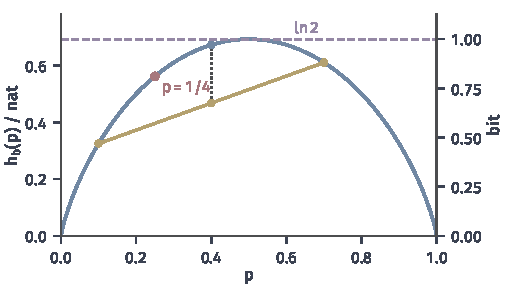
\includegraphics[width=86mm]{figures/07-probability/04-distribution-analysis/matplotlib/info-binary-entropy/figure.pdf}
  \caption{二元熵函数$h_{\mathrm{b}}(p)$（蓝），左轴nat、右轴bit。紫虚线为上界$\ln2$，在$p=\tfrac12$处达到。黄色弦连接$p=0.1$与$p=0.7$两点，其中点$0.470$低于曲线在$p=0.4$处的值$0.673$，体现凹性。红点为$p=\tfrac14$。}
  \label{fig:info-binary-entropy}
\end{BookInlineFigure}

图~\ref{fig:info-binary-entropy}中，$h_{\mathrm{b}}$在两端为零，对应确定的结果；在$p=\tfrac12$处取最大值$\ln2$，对应公平硬币；曲线关于$p=\tfrac12$对称，因为交换$0$与$1$不改变熵。端点附近曲线很陡：$h_{\mathrm{b}}'(p)=\ln\frac{1-p}{p}\to+\infty$（$p\downarrow0$），概率从$0$略微增加，熵增加得比概率快得多。第~\ref{sec:info-continuity}节讨论熵的连续性时会用到这一点。

三个取值的情形可以画在概率单纯形上。图~\ref{fig:info-simplex-entropy}中三角形的每个点是一张概率表，顶点是确定结果，中心是均匀分布。等熵线围绕中心形成一圈圈闭曲线：越靠近中心越不确定。

\begin{BookInlineFigure}
  \centering
  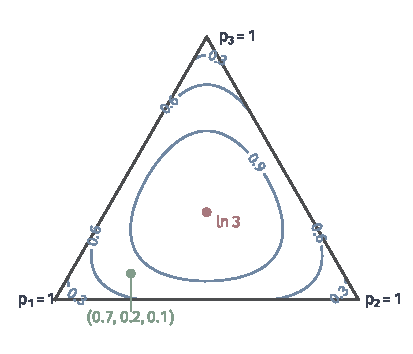
\includegraphics[width=70mm]{figures/07-probability/04-distribution-analysis/matplotlib/info-simplex-entropy/figure.pdf}
  \caption{三点分布$(p_1,p_2,p_3)$的熵在概率单纯形上的等值线（蓝，数值为nat）。顶点熵为$0$，红点为均匀分布，熵$\ln3\approx1.099$；绿点为$(0.7,0.2,0.1)$，熵约$0.802$ nat。超水平集$\{H\geq c\}$是凸集，对应熵的凹性。}
  \label{fig:info-simplex-entropy}
\end{BookInlineFigure}

\paragraph{可数取值}
取值可数无穷时，式~\eqref{eq:info-entropy}是非负项级数，可能收敛，也可能发散。几何分布$\operatorname{Geom}(\tfrac12)$取值$k=1,2,\dots$，概率$2^{-k}$，自信息$k\ln2$，于是
\[
  H(X)=\sum_{k\geq1}2^{-k}\,k\ln2=2\ln2,
\]
相当于平均问两题。

熵也可以是无穷。取$k\geq2$，$p_X(k)=c/(k(\ln k)^2)$，其中$c$使概率之和为$1$；由积分判别法，$\sum_{k\geq2}1/(k(\ln k)^2)$收敛，所以这样的$c>0$存在。这时
\[
  -\ln p_X(k)=\ln k+2\ln\ln k-\ln c\geq\ln k-\ln c.
\]
对充分大的$k$，$2\ln\ln k\geq0$，所以熵的级数从某项起不小于
\[
  \sum_k\frac{c}{k(\ln k)^2}\bigl(\ln k-\ln c\bigr)\geq\sum_k\frac{c}{k\ln k}-\ln c\sum_k\frac{c}{k(\ln k)^2},
\]
其中第一项发散，第二项有限，故$H(X)=+\infty$。这个分布的质量衰减得足够快，使概率之和有限，却不够快，使平均自信息有限。

所以定理~\ref{thm:info-entropy-range}的上界不能移用到可数字母表：$\ln m$随$m\to\infty$趋于无穷，并不给出有限上界。凹性在熵有限的分布之间仍然成立，因为证明只用到逐项的不等式；但涉及熵之差的公式，都要先核对相关的熵有限。

\subsection{微分熵}
\label{sec:info-differential-entropy}

连续随机变量的每个取值概率都是零，自信息全是无穷大，式~\eqref{eq:info-entropy}不能直接用。一个自然的替代是把概率质量换成密度：密度是单位长度上的概率质量，对密度取负对数再按分布平均。

\begin{definition}[微分熵]
\label{def:info-differential-entropy}
设随机变量$X$有密度$f_X$。若$f_X\ln f_X$在$\mathbb{R}$上可积，称
\begin{equation}
  h(X)=-\int_{\mathbb{R}}f_X(x)\ln f_X(x)\,\mathrm{d}x=\mathbb{E}[-\ln f_X(X)]
  \label{eq:info-differential-entropy}
\end{equation}
为$X$的\term{微分熵}（differential entropy），在$\{f_X=0\}$上约定被积函数为$0$。随机向量$\bm{X}$有联合密度时，同样定义$h(\bm{X})$。
\end{definition}

定义里要求$f_X\ln f_X$可积（即$f_X\lvert\ln f_X\rvert$的积分有限），是为了排除两种情形。离散熵的各项非负，最坏只是$+\infty$；而密度可以大于$1$，$-\ln f_X$有正有负，正部与负部的积分可能都发散，这时“$\infty-\infty$”没有意义。若只有一部分发散，可以约定$h(X)=+\infty$或$-\infty$，本章不使用这种扩展。

\paragraph{几个密度的微分熵}
均匀分布$\operatorname{Unif}(0,a)$的密度在$(0,a)$上为$1/a$，所以
\[
  h(X)=-\int_0^a\frac1a\ln\frac1a\,\mathrm{d}x=\ln a.
\]
$a<1$时它是负数。$\operatorname{Unif}(0,\tfrac12)$的微分熵是$-\ln2$，这不意味着“不确定性为负”，而是说密度$2$大于$1$。

正态分布$\mathcal{N}(\mu,\sigma^{2})$的对数密度是
\[
  \ln f_X(x)=-\frac12\ln(2\pi\sigma^{2})-\frac{(x-\mu)^{2}}{2\sigma^{2}}.
\]
取负号再按$X$平均，利用$\mathbb{E}[(X-\mu)^{2}]=\sigma^{2}$，得到
\begin{equation}
  h(X)=\frac12\ln(2\pi\sigma^{2})+\frac12=\frac12\ln(2\pi\mathrm{e}\sigma^{2}).
  \label{eq:info-gaussian-entropy}
\end{equation}
$\sigma=1$时约为$1.419$ nat。同样算出指数分布$\operatorname{Exp}(\lambda)$的微分熵：$-\ln f_X(x)=-\ln\lambda+\lambda x$，平均为$1-\ln\lambda$。

\paragraph{坐标尺度的作用}
把变量放大，密度就按比例变矮。设$a\neq0$，$Y=aX+b$，由第~\ref{chap:random-variable-transformations}章的换元公式，$f_Y(y)=f_X((y-b)/a)/\lvert a\rvert$。于是
\[
  -\ln f_Y(Y)=-\ln f_X(X)+\ln\lvert a\rvert,
\]
两边取期望，得到
\begin{equation}
  h(aX+b)=h(X)+\ln\lvert a\rvert.
  \label{eq:info-differential-entropy-scale}
\end{equation}
平移不改变微分熵，伸缩改变$\ln\lvert a\rvert$。图~\ref{fig:info-diff-entropy-scale}把这一点画了出来：宽度每加倍，高度减半，微分熵增加$\ln2$。

\begin{BookInlineFigure}
  \centering
  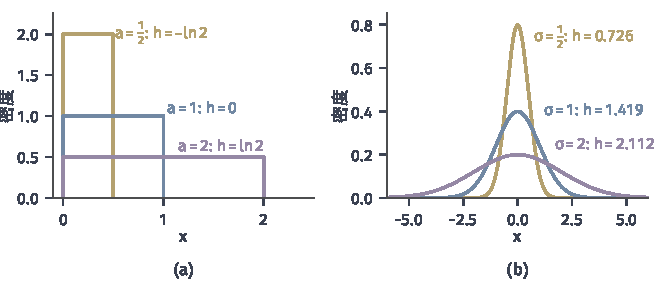
\includegraphics[width=112mm]{figures/07-probability/04-distribution-analysis/matplotlib/info-diff-entropy-scale/figure.pdf}
  \caption{微分熵随尺度变化。(a)$\operatorname{Unif}(0,a)$，$a=\tfrac12,1,2$（黄、蓝、紫），微分熵为$\ln a$。(b)$\mathcal{N}(0,\sigma^{2})$，$\sigma=\tfrac12,1,2$，微分熵按式~\eqref{eq:info-gaussian-entropy}计算，以nat计。宽度加倍时两组都增加$\ln2\approx0.693$。}
  \label{fig:info-diff-entropy-scale}
\end{BookInlineFigure}

式~\eqref{eq:info-differential-entropy-scale}揭示了微分熵与离散熵的根本不同。同一个长度用米记录是$X$，用厘米记录是$100X$，两者包含的关于这次测量的信息完全一样，微分熵却相差$\ln100$。离散熵没有这个问题：对取值作任何一一变换，概率表不变，熵不变。微分熵依赖坐标，只有在固定坐标下比较才有意义。更一般地，对严格单调可微的$g$，$Y=g(X)$满足$h(Y)=h(X)+\mathbb{E}[\ln\lvert g'(X)\rvert]$（右端各项有限时），推导与上面相同。

\paragraph{与量化后离散熵的关系}
微分熵可以从离散熵得到，只是要减去一个随精度增长的量。把实轴按宽度$\Delta>0$分成格子$[k\Delta,(k+1)\Delta)$，只记录$X$落在哪一格，得到离散变量$X_{\Delta}$，概率$p_k=\mathbb{P}(k\Delta\leq X<(k+1)\Delta)$。

若$f_X$连续，由积分中值定理，每格中有一点$\xi_k$使$p_k=f_X(\xi_k)\Delta$。代入离散熵并利用$\sum_kp_k=1$，得到
\[
  H(X_{\Delta})=-\sum_kf_X(\xi_k)\Delta\ln f_X(\xi_k)-\ln\Delta.
\]
右端第一项是$-\int f_X\ln f_X\,\mathrm{d}x$的一个Riemann和。若这个和在$\Delta\to0$时收敛到积分，就有
\begin{equation}
  H(X_{\Delta})+\ln\Delta\to h(X),\qquad\Delta\to0.
  \label{eq:info-quantized-entropy}
\end{equation}

$-\ln\Delta$是“把结果确定到精度$\Delta$”的代价：每把格子缩小一半，就要多回答一个是非题。连续结果要完全确定需要无穷多个是非题，离散熵趋于无穷；微分熵是减去这部分以后剩下的有限部分，所以它依赖格子的单位。$X\sim\operatorname{Unif}(0,1)$、$\Delta=1/n$时，$n$个格子等概率，$H(X_{\Delta})=\ln n$恰好等于$h(X)-\ln\Delta=0+\ln n$。

\begin{BookInlineFigure}
  \centering
  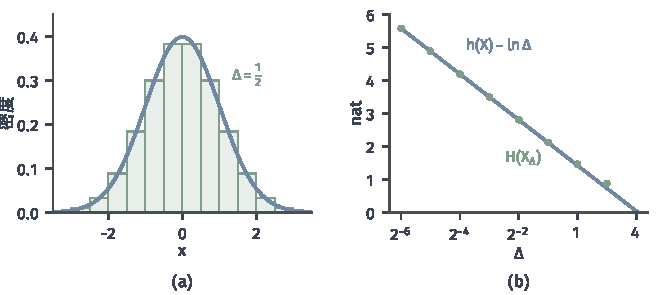
\includegraphics[width=112mm]{figures/07-probability/04-distribution-analysis/matplotlib/info-quantization/figure.pdf}
  \caption{标准正态变量的量化。(a)密度（蓝）与$\Delta=\tfrac12$时各格的概率除以格宽（浅绿柱）。(b)量化后离散熵$H(X_{\Delta})$的精确值（绿点）与$h(X)-\ln\Delta$（蓝线），$h(X)\approx1.419$ nat，横轴为对数刻度。差$H(X_{\Delta})+\ln\Delta-h(X)$在$\Delta=1,\tfrac12,\tfrac14$时约为$0.040,0.010,0.0026$。}
  \label{fig:info-quantization}
\end{BookInlineFigure}

图~\ref{fig:info-quantization}对标准正态变量逐格计算了$H(X_{\Delta})$。格子较宽时两者有可见的差距，$\Delta$每减半，差距约缩小为四分之一。

式~\eqref{eq:info-quantized-entropy}不是对任意密度都成立。上面的推导用到两件事：$f_X\ln f_X$的Riemann和收敛到积分，以及实轴无界时尾部格子的贡献可以忽略。密度连续且$f_X\ln f_X$在有界区间上Riemann可积时，有界区间上的部分成立；无界区间还需要控制尾部，读者可查阅~\scite{math-cover2006information}。密度剧烈振荡或尾部很重时，两边可能不相符。因此，微分熵与量化熵是两个不同的量，前者不是后者的极限值，而是后者减去$-\ln\Delta$后的极限，并且这个联系要单独核对条件。
